% !TeX spellcheck = en_GB
\documentclass[11pt]{article}

\usepackage[type1]{libertine}
\usepackage[a4paper]{geometry}
\usepackage{amsmath, amsthm, amssymb} 
\usepackage{parskip}
\usepackage{tabularx}
\usepackage[english]{babel}
\usepackage{enumitem}
\usepackage{gensymb}
\usepackage{bm}
\usepackage{graphicx}
\usepackage{xcolor}
\usepackage{float}
\usepackage{wrapfig}
\usepackage[makeroom]{cancel}
\usepackage{multicol}
\usepackage{commath} % Provides good differentials
\usepackage{siunitx} % Provides good units
\usepackage{nicefrac}

\usepackage[titletoc,title,toc,page]{appendix}
\usepackage{hyperref}
\hypersetup{
	pdftitle={Period of a Pendulum as an example of Simple Harmonic Motion},
	pdfauthor={Sun Yudong},
	bookmarksnumbered=true,
	bookmarksopen=true,
	bookmarksopenlevel=2,
	pdfstartview=Fit,
	pdfpagemode=UseOutlines,
	colorlinks=true,
	linkcolor=black,
	filecolor=magenta,      
	urlcolor=blue
}

\newcommand{\uvec}[1]{\boldsymbol{\hat{\textbf{#1}}}}
\newcommand{\solution}[1]{\textbf{Solution: } #1 \hspace{5mm}}

\newenvironment{multicolFigure}
{\par\medskip\noindent\minipage{\linewidth}}
{\endminipage\par\medskip}
% https://tex.stackexchange.com/questions/12262/multicol-and-figures

%\newenvironment{amatrix}[1]{%
%	\left(\begin{array}{@{}*{#1}{c} | c@{}}
%	}{%
%	\end{array}\right)
%}						% https://tex.stackexchange.com/a/2238
%\usepackage{blkarray}	% https://tex.stackexchange.com/a/59519
%\usepackage{mathtools}	% https://tex.stackexchange.com/a/103993

\title{Period of a Pendulum\\{\normalsize As an example of Simple Harmonic Motion}}
\author{Sun Yudong}

\begin{document}
	\maketitle
	
	\begin{wrapfigure}{r}{3.5cm}
		\vspace{-0.5cm}
		\centering
		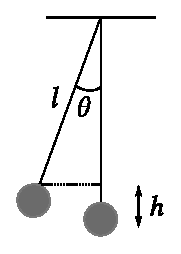
\includegraphics[height=4cm]{pendulum.eps}
		\vspace{-1cm}
	\end{wrapfigure}
	
	This derivation requires that you are already familiar with calculus, circular motion and simple harmonic motion. 
	
	Presented here are 2 ways we can derive the equations that govern the motion of a simple pendulum. These concepts can, of course, be extended to more complex systems.
	
	\subsection*{Analysis of Total Energy}
	We first write out the energy of the system:
	\begin{align*}
	E &= U + \text{KE} \\
	&= mgh + \frac{1}{2}mv^2 \\
	&= mg(l - l\cos \theta ) + \frac{1}{2}m\left(r\omega\right)^2 \\
	&= mgl(1 - \cos \theta ) + \frac{1}{2}m\left(l\dod{\theta}{t}\right)^2
	\end{align*}
	Now we differentiate the expression with respect to time:
	\begin{align*}
	\dod{E}{t} &= mgl\left[\dod{}{t}(1 - \cos \theta)\right] + \frac{1}{2}ml^2\left[\dod{}{t}\left(\dod{\theta}{t}\right)^2\right] \\
	&= mgl\left[\sin \theta \cdot \dod{\theta}{t}\right] + \frac{1}{2}ml^2\left[2\left(\dod{\theta}{t}\right)\left(\dod[2]{\theta}{t}\right)\right] \\
	&= ml\dod{\theta}{t}\left[g\sin \theta + l\dod[2]{\theta}{t}\right]
	\end{align*}
	Since total energy is conserved, the rate of change of $E$ must be zero:
	\begin{align*}
	0 &= ml\dod{\theta}{t}\left[g\sin \theta + l\dod[2]{\theta}{t}\right] \\
	&= g\sin \theta + l\dod[2]{\theta}{t} \\
	\dod[2]{\theta}{t} &= -\frac{g}{l} \sin \theta
	\end{align*}
	For sufficiently small $\theta$, $\sin \theta \approx \theta$:
	\begin{equation}
	\dod[2]{\theta}{t} = -\frac{g}{l}\theta \label{eqn:pendulum}
	\end{equation}
	\subsection*{Analysis of Restoring Forces}
	\begin{wrapfigure}{r}{3.5cm}
		\vspace{-0.5cm}
		\centering
		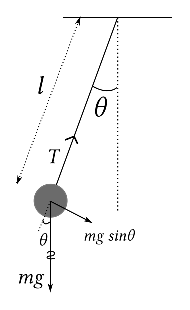
\includegraphics[width=3cm]{pendulum-restoring.eps}
		\vspace{-2cm}
	\end{wrapfigure}
	
	We can also obtain Equation \eqref{eqn:pendulum} by considering the restoring forces on a point mass at the end of a pendulum:
	\begin{align*}
	F_{\text{net}} &= -mg \sin \theta \\
	a_{\text{restoring}} &= -g\sin \theta 
	\end{align*}
	which has a corresponding angular form of:
	\begin{align*}
	\left(a = r \alpha = \right)~ l \dod[2]{\theta}{t} &= -g\sin \theta \\ 
	\dod[2]{\theta}{t} &= -\frac{g}{l}\sin\theta
	\end{align*}
	For sufficiently small $\theta$, $\sin \theta \approx \theta$:
	\begin{equation*}
	\dod[2]{\theta}{t} = -\frac{g}{l}\theta \tag{\ref{eqn:pendulum}}
	\end{equation*}
	
	\subsection*{Relating to Simple Harmonic Motion}
	Now we compare the obtained Equation \eqref{eqn:pendulum} to the general solution/defining equation of Simple Harmonic Motion:
	\begin{equation}
	a=-\omega^2x \label{eqn:shm}
	\end{equation}
	
	Since the angular form and the tangential form of all dynamics and kinematics equations are proportional by a factor of radius $r$, it doesn't really matter which regime we are working in.
	
	Comparing \eqref{eqn:pendulum} and \eqref{eqn:shm}, we realize that:
	\begin{equation*}
	\omega^2 = \frac{g}{l} ~~~\implies ~~~ \omega = \sqrt{\frac{g}{l}}
	\end{equation*}
	Using this relationship, we can then find the period of the oscillation:
	\begin{flalign*}
	&& T = 2\pi \sqrt{\frac{l}{g}} && \left(\omega = \frac{2\pi}{T}\right)
	\end{flalign*}
	
	\subsection*{Proving something follows Simple Harmonic Motion}
	The energy way of tackling this problem is actually a simple and  general way to prove that the motion of a certain object follows that of simple harmonic motion:
	\begin{enumerate}
		\item Write an expression for the total energy of the system.
		\item Differentiate the expression with respect to time. Since total energy $E_{\text{tot}}$ is conserved, the rate of change of $E_{\text{tot}}$ is zero with respect to time
		\item Solve for the acceleration of the system. If the motion does indeed follow simple harmonic motion, then the acceleration of the system would be in the form of:
		\begin{equation*}
		\dod[2]{x}{t} = a =-\omega^2x
		\end{equation*}
	\end{enumerate}
	We can then find the period and frequency of this oscillation from the $\omega$: 
	\begin{equation*}
	\omega = 2\pi f = \frac{2\pi}{T}
	\end{equation*}
	
	Note that when writing the energy expression for more complex pendulums, it would be more useful to use the moment of inertia $I$ and its corresponding $$\text{KE} = \frac{1}{2} I \omega^2$$ (where $\omega$ is the angular velocity) instead of mass $m$ and the tangential velocity $v$. 
	
	This is because, while the tangential velocity $v$ for every particle along a rigid pendulum stick is different, the angular momentum $\omega$ is the same for the entire stick.
\end{document}